\subsection{Проблемы производительности при операциях случайного добавления}
\label{sec:optimization:random_updates}

Операции случайного добавления (\emph{random insertion updates}) – такие операции обновления предиката с помощью дельта-предиката, которые исходя из упорядоченных ключей в структуре представления на диске затрагивают изменения в слишком большом количестве страниц.

Например, у нас после выполнения недельного скрипта сохранилась информация о продажах за некоторую неделю. Дельты для них:

\begin{lstlisting}[language=Prolog]
^sales["Sprite", "Belarus", "20160917"]=9.6
^sales["Sprite", "Russia", "20160917"]=2.0
^sales["Maple syrup", "Belarus", "20160917"]=4.0
\end{lstlisting}

Посмотрим, что происходит при обновлении предиката \lstinline{^sales}:

\begin{enumerate}
  \item инициализация итераторов (рисунок \ref{fig:optimization:random_updates:iter_init});
  \item выравнивание итераторов – установка на первую страницу (рисунок \ref{fig:optimization:random_updates:iter_align_first});
  \item обновление записи (рисунок \ref{fig:optimization:random_updates:iter_update_fact});
  \item перемещение итераторов далее (рисунок \ref{fig:optimization:random_updates:iter_advance});
  \item обновление следующих записей и т.д.
\end{enumerate}

\begin{figure}
	\centering
	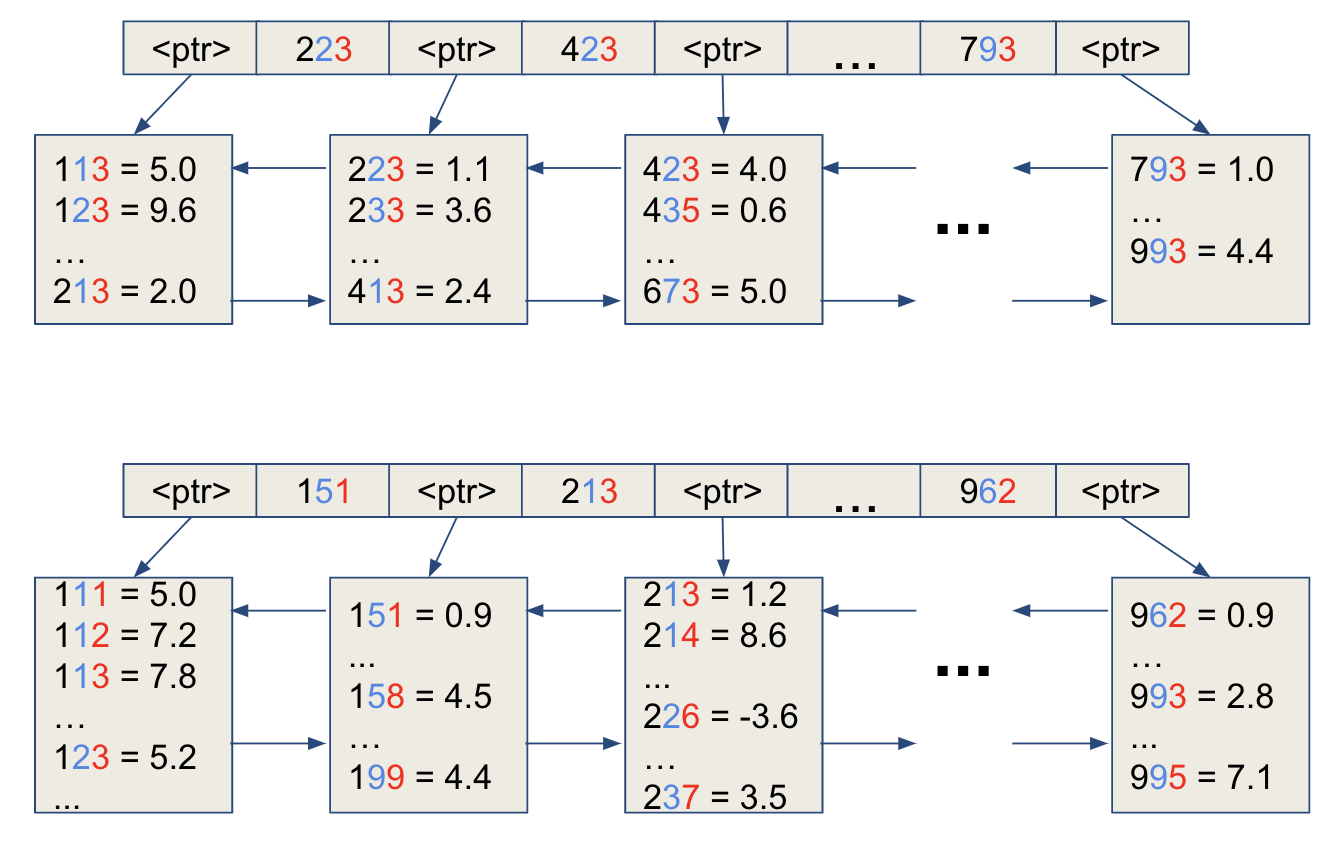
\includegraphics[scale=0.3]{update_0.png}
	\caption{Начальные значения в предикатах \lstinline{^sales} и \lstinline{sales}}
	\label{fig:optimization:random_updates:iter_init}
\end{figure}
\begin{figure}
	\centering
	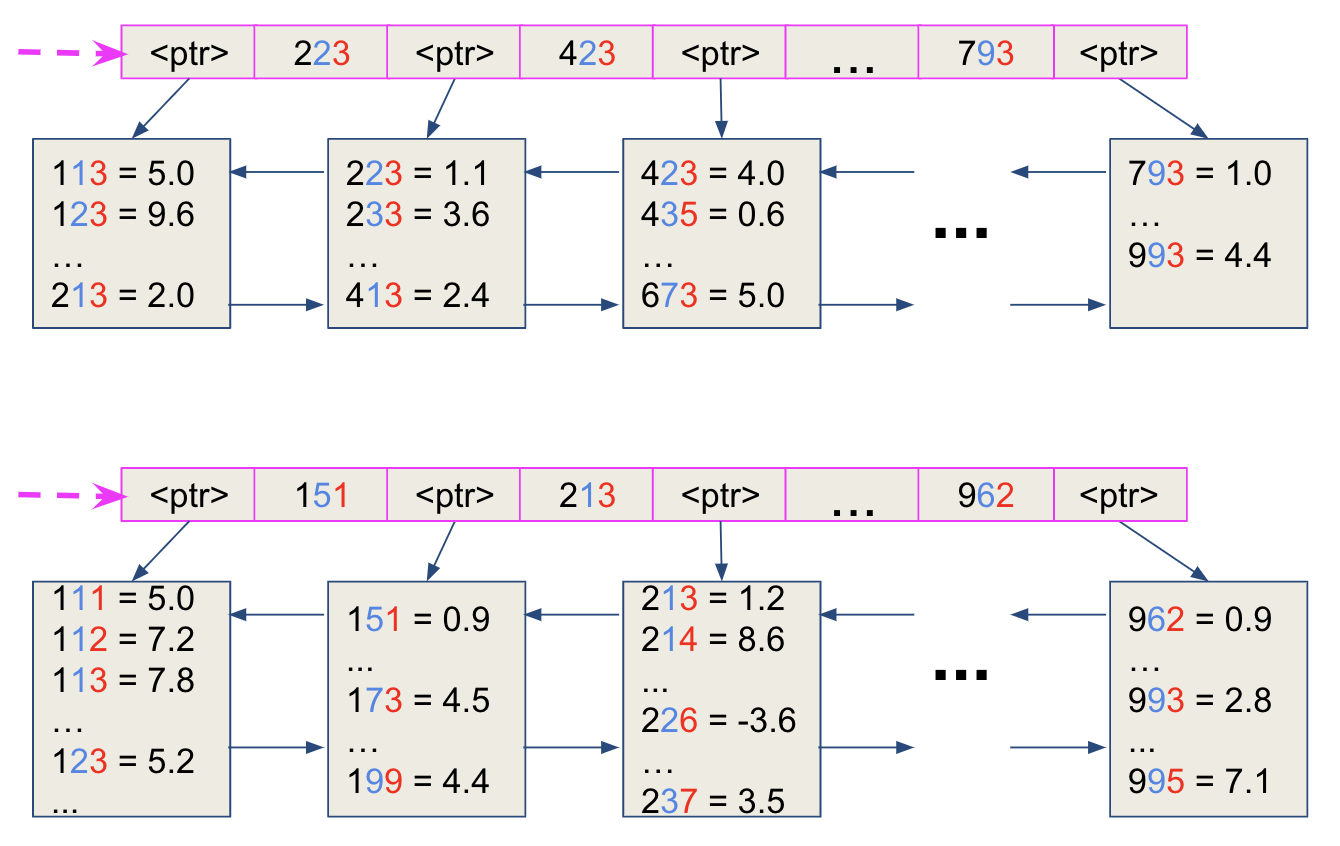
\includegraphics[scale=0.3]{update_1.png}
	\caption{Выравнивание итераторов по первым страницам}
	\label{fig:optimization:random_updates:iter_align_first}
\end{figure}
\begin{figure}
	\centering
	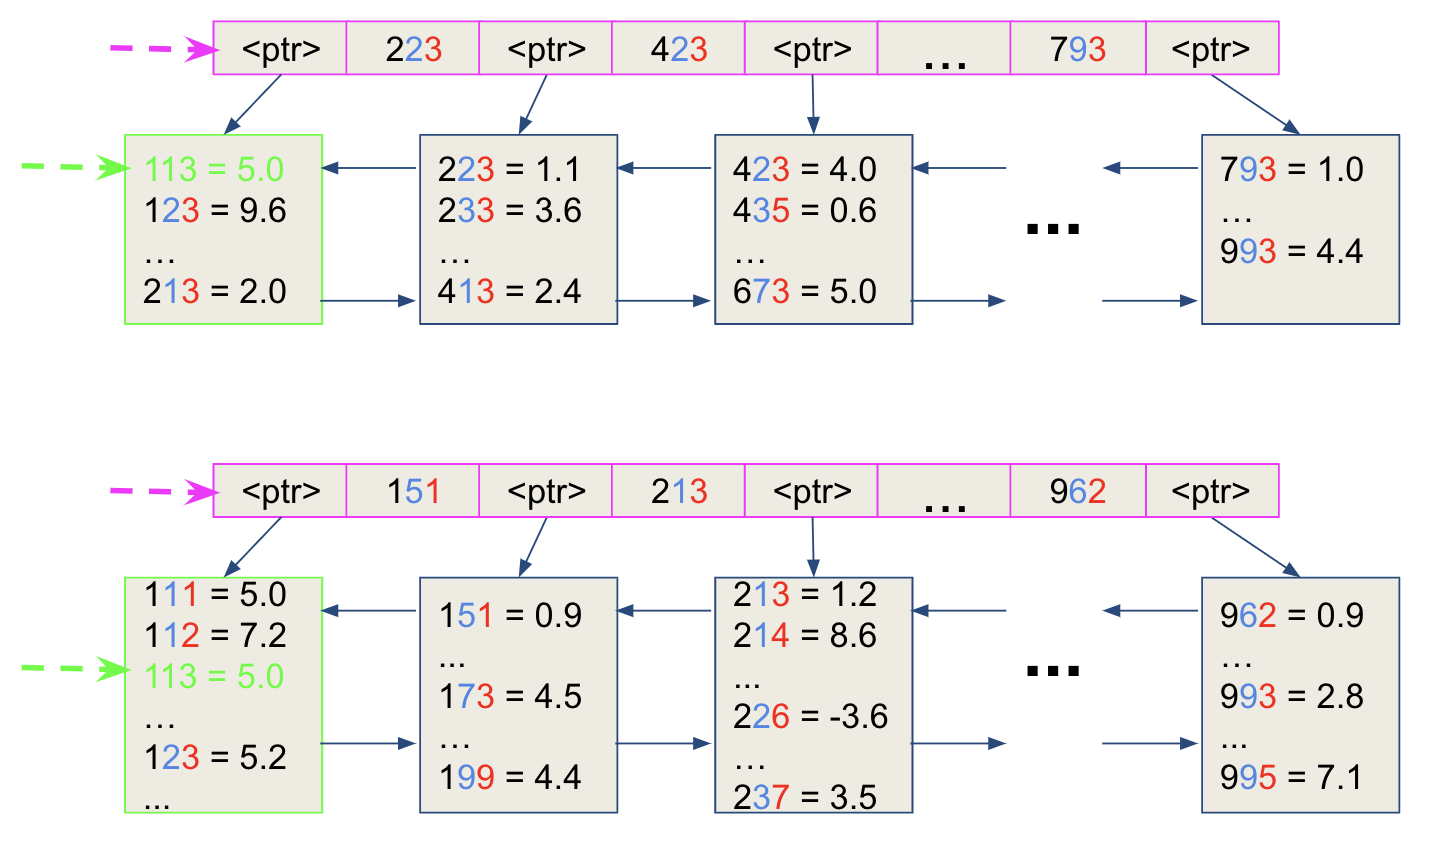
\includegraphics[scale=0.3]{update_2.png}
	\caption{Нахождение нужной записи и ее обновление}
	\label{fig:optimization:random_updates:iter_update_fact}
\end{figure}
\begin{figure}
	\centering
	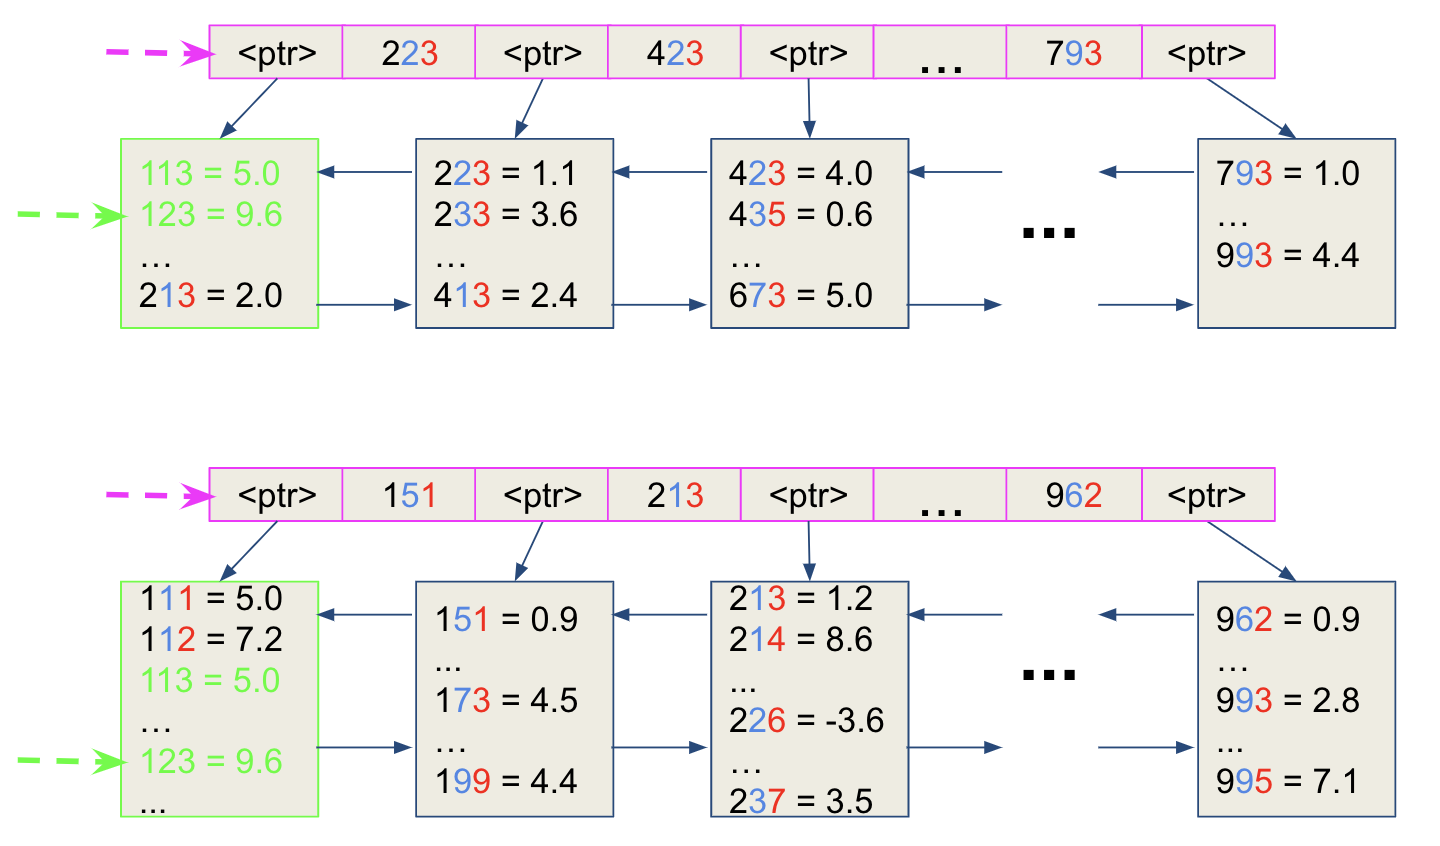
\includegraphics[scale=0.3]{update_3.png}
	\caption{Перемещение итераторов далее для обновления следующих записей}
	\label{fig:optimization:random_updates:iter_advance}
\end{figure}

Заметим некоторые моменты, присущие обновлению записей:

\begin{itemize}
  \item обновление затронуло оба предиката \lstinline{sales} и \lstinline{^sales};
  \item если размер предикатов большой, обновление распараллеливается и работает с помощью множественных итераторов;
  \item ситуация может ухудшиться, если в процессе обновления будут строгие добавления новых записей, что может привести к многократному увеличению размеров листьев и, как следствие, приходится их разбивать на более мелкие. Именно поэтому стоит разбивать, например, не по \lstinline{(sku, store, week)}, а по \lstinline{(week, store, sku)}.
\end{itemize}
